%%%%%%%%%%%%%%%%%%%%%%%%%%%%%%%%%%%%%%%%%%%%%%%%%%%%%%%%%%%%%%%%%%%%%%%
%%%                           SECTION II
%%%%%%%%%%%%%%%%%%%%%%%%%%%%%%%%%%%%%%%%%%%%%%%%%%%%%%%%%%%%%%%%%%%%%%

\chapter{\uppercase {The \textit{Ube3a} antisense transcript undergoes extensive processing and is spatiotemporally regulated in the brain}}\label{chapter2}

\subsubsection*{Abstract}

Human chromosome 15q11-q13 contains a cluster of imprinted genes that are associated with a number of neurodevelopmental disorders that exhibit non-Mendelian patterns of inheritance due to genomic imprinting, including Angelman syndrome (AS), Dup15q syndrome, and Prader-Willi syndrome (PWS). AS is caused by loss of the maternally inherited \textit{UBE3A} allele, whereas PWS is caused by the loss of the paternally inherited \textit{SNORD116} snoRNAs, which are expressed as part of a long polycistronic transcription unit (PTU) comprised of \textit{SNRPN}, additional snoRNA clusters, and the \textit{UBE3A} antisense transcript (\textit{UBE3A-AS}). The PTU is imprinted with paternal-specific expression, and its antisense portion exclusively expressed in neurons. As a result, \textit{UBE3A} is imprinted in neurons and biallelically expressed in all other cell-types. Why \textit{UBE3A-AS} evolved to imprint \textit{UBE3A} in neurons is largely unknown. In this study, we examined the transcriptional profiles and processing of the mouse and human antisense transcripts towards understanding the functional significance of \textit{UBE3A} imprinting by \textit{UBE3A-AS}. Our findings show that the \textit{UBE3A-AS} is extensively processed via 5' capping, 3' polyadenylation, and alternative splicing, giving rise to a myriad of transcripts that are spatiotemporally regulated. Based on our findings, we propose that processing of the \textit{UBE3A-AS} generates a diverse repertoire of regulatory RNAs in neurons.

\section{Introduction}

Human chromosome 15q11-q13 contains a cluster of genes that are associated with a number of neurodevelopmental disorders exhibiting non-Mendelian patterns of inheritance due to genomic imprinting. Angelman syndrome (AS) - characterized by intellectual disability, ataxia, epilepsy, and an atypical happy disposition - is caused by mutations or epimutations leading to loss-of-function or loss-of-expression of the maternally inherited ubiquitin protein ligase E3A (\textit{UBE3A}) gene \cite{Yamasaki2003,Dindot2008,Sutcliffe1997}. Maternal-derived interstitial or isodicentric copy number gains of 15q11-q13 cause Dup15q syndrome, which is characterized by intellectual disability, ataxia, epilepsy, sleep disorder, and autism spectrum disorder \cite{Battaglia2008,Battaglia1997}. Although Dup15q is a contiguous gene disorder, overexpression of UBE3A in the brain is believed to be the principal mechanism underlying the symptoms associated with the condition \cite{Scoles2011}. Paternally inherited deletions of 15q11-q13, namely those involving the C/D box small nucleolar RNA (snoRNA) \textit{SNORD116}, cause Prader-Willi syndrome (PWS), which is characterized by dysregulated hunger and satiety, thermoregulation, sleep disorder, and behavioral issues \cite{Sahoo2008}.

Genomic imprinting of the 15q11-q13 region is regulated by the AS and PWS imprinting centers (AS-IC and PWS-IC) \cite{Buiting1999,Buiting1998,Kantor2006,Chamberlain2001,Buiting2001}. Studies to date indicate that the AS-IC negatively regulates the PWS-IC \cite{Kantor2006}, while the PWS-IC functions as an enhancer element that positively regulates the expression of genes in the region \cite{Nicholls2001}. On the maternal chromosome, the AS-IC is active and thus represses the expression of the genes controlled by the PWS-IC. On the paternal chromosome, repressive histone modifications and DNA methylation inactivate the AS-IC allowing for the PWS-IC to regulate the expression of its target genes on the paternal chromosome, which including the polycistronic transcriptional unit (PTU) comprised of \textit{SNURF/SNRPN}, and clusters of tandemly repeated C/D small nucleolar RNAs (\textit{SNORD107, SNORD64, SNORD108, SNORD109A, SNORD116}, and \textit{IPW}. In the brain, transcription extends downstream of \textit{IPW} to include additional tandemly duplicated snoRNAs (\textit{SNORD115} and \textit{SNORD109B}) and the \textit{UBE3A} antisense transcript (\textit{UBE3A-AS}, also known as \textit{UBE3A-ATS}). Likewise, the mouse functional equivalent of the PWS-IC regulates the expression of a PTU comprised of \textit{Snurf/Snrpn}, clusters of C/D box snoRNAs (\textit{Snord64, Snord116, Snord115}, \textit{Ipw}, and \textit{Ube3a-AS}. But unlike in humans, expression of \textit{Snord116, Ipw, Snord115,} and \textit{Ube3a-AS} is brain-specific \cite{Landers2004,LeMeur2005}. As such, the imprinting of \textit{UBE3A/Ube3a} is brain-specific, and aside from this role in imprinting there is no other function ascribed to it. 

Studies in mouse and human have shown that expression of \textit{Ube3a-AS/UBE3A-AS} transcript is both necessary and sufficient to silence expression of the paternal \textit{Ube3a/UBE3A} allele \textit{in cis } \cite{Meng2013,Martins-Taylor2014}. But unlike most imprinted genes regulated by an antisense transcript, the \textit{Ube3a-AS/UBE3A-AS} is believed to inhibit transcriptional elongation rather than transcriptional initiation, as the paternal \textit{Ube3a} allele is modified with active epigenetic modifications, bound by RNA polymerase II, and transcribed to a region in intron 4 \cite{Meng2013}. As such, Meng \textit{et al.} (2013) proposed a collision model for the imprinting of \textit{Ube3a} in neurons, wherein \textit{Ube3a} and \textit{Ube3a-AS} expression decreases within intron 4 due to collision of the RNA polymerases. This model, however, conflicts with reports detecting \textit{Ube3a-AS} expression upstream \textit{Ube3a} \cite{Numata2011}. As such, this study sets out to investigate the expression profile of \textit{Ube3a-AS/UBE3A-AS} as a means to understand the function of imprinting in neurons. Here, were report that \textit{Ube3a-AS/UBE3A-AS} is a remarkably complex transcript that is extensively processed through 5' capping, alternative splicing, and 3' polyadenylation, which are differentially regulated among brain regions and during brain development.

\section{Materials \& Methods}
\section*{Bioinformatics}
\subsection{Public data, genomes and annotations}
\subsubsection{Publicly available data}
The analysis performed in this chapter was conducted with publicly available data downloaded from the European Nucleotide Archive, and can be viewed by the accession number (\url{http://www.ebi.ac.uk/ena/data/view/<accession>}). Mouse tissue data was from 8 wk adults \cite{Pervouchine2015}, while adult human data was of unknown age and origin for Human Protein Atlas (ERP003613) \cite{Uhlen2015}, and an average of 52.3 $\pm$ 7.9 year-old for the SRP072463 study \cite{Lin2016}. The cellular populations in the mouse cerebral cortex dataset were purified with various purification methods \cite{Zhang2014}. Temporal hippocampal RNA-seq datasets were extracted from E18, P1, P10 and P30 mice \cite{You2015}. A breakdown of tissue types, strain, and accession numbers is supplied in \textbf{APPENDIX B, Table \ref{tableB:1}} for mouse data and \textbf{APPENDIX B, Table \ref{tableB:2}} for human data. A complete list of publicly available RNA-seq datasets used in this chapter is provided in \textbf{Table \ref{table2:1}}. 

%%%%%%%%%%%%%%%%%%%%%%%%%%%%%%%%%%%%%%%%%%%%%%%%%%%%%%
\begin{longtabu} {X[.7,c]X[2,c]X[0.5,c]X[0.6,c]X[1,c]}
  \caption{Public Data: RNA-seq information}\\
  \label{table2:1}\\
  \toprule
  \textbf{Study} & \textbf{Instrument} & \textbf{Layout} & \textbf{Stranded} & \textbf{Species}\\
  \midrule
  \endhead
  ERP000591 & Illumina Genome Analyzer & PE & No  & \textit{Mus musculus}\\
  SRP012040 & Illumina HiSeq 2000      & PE & Yes & \textit{Mus musculus}\\
  SRP033200 & Illumina HiSeq 2000      & PE & No  & \textit{Mus musculus}\\
  SRP048593 & Illumina HiSeq 2500      & SE & Yes & \textit{Mus musculus}\\
  ERP003613 & Illumina HiSeq 2000      & PE & No  & \textit{Homo sapiens}\\
  SRP072463 & Illumina HiSeq 2000      & PE & Yes & \textit{Homo sapeins}\\
  \bottomrule
\end{longtabu}
%%%%%%%%%%%%%%%%%%%%%%%%%%%%%%%%%%%%%%%%%%%%%%%%%%%%%%

\subsubsection{Genomes and annotation sets}
Throughout this work, we used the February 2009, Genome Reference Consortium Human Reference 37 (GRCh37, hg19) human genome assembly \cite{Lander2001} and the July 2007 finished mouse genome NCBI Build 37 assembly \cite{Chinwalla2002} (mm9). Annotations were collected from Illumina iGenomes collection for hg19 and mm9 last downloaded from UCSC on July 17, 2015 \cite{Rosenbloom2014}.

\subsubsection{PolyA-seq data}
PolyA-seq data files from Derti \emph{et al.}, 2012 \cite{Derti2012} were downloaded from UCSC. The sites clustered BED files from mouse and human (hg19) were separated by strand with \texttt{awk} (version 4.0). These files were than viewed with IGV (version 2.3.90 \cite{Thorvaldsdottir2013,Robinson2011}).

\subsubsection{CAGE-seq data}
CAGE (Capped Analysis of Gene Expression) sequencing bed files generated from the FANTOM5 consortium \cite{Lizio2015} were downloaded from \url{http://fantom.gsc.riken.jp/5/datafiles/latest/extra/CAGE_peaks/}. Similar to polyA-seq data, files were separated by strand with \texttt{awk} and viewed in IGV.

\subsection{Data processing}
Quality of downloaded raw fastq files were checked with FastQC \cite{Andrews_Fastqc} (version 0.11.5). As no read files failed initial quality control, adapter sequences and low quality reads (quality score $\leq$ 3) were trimmed with Trimmomatics \cite{Bolger2014} (version 0.36). Using the program's TruSeq3-PE-2.fa adapter file, and minimal length of 25. These trimmed paired- and single-end reads were used by Hisat2 \cite{Pertea2016,Kim2015} (version 2.0.4) to align to chromosome 15 (chr15) for human and chromosome 7 (chr7) for mouse data. The alignment was assisted with Hisat2 python provide extraction scripts for splice sites and exons within chr15 and chr7, human and mouse alignments respectively. The SAM file outputs were directly pipped into SAMtools \cite{Li2009} (version 1.3.1) to convert to BAM format (\texttt{samtools view}) and sorted (\texttt{samtools sort}) outputting only sorted BAM files to be indexed (\texttt{samtools index}) and merged (\texttt{samtools merged}). The sorted BAM files were assembled with StringTie \cite{Pertea2015,Pertea2016} (version 1.3.3). Annotation files using stranded, high-depth reads (SRP01204, SRP072463) were generated via \texttt{stringtie} \textit{de novo} method for mouse and human datasets. These GTF annotation files were merged with \texttt{stringtie -{}-merge} using FPKM thresholds of 5 and 10 for mouse and human data respectively. Mouse data was additionally restricted with isoform fraction equal to 0.05. These annotations were used for downstream analysis like \texttt{featureCounts} \cite{Liao2013b} - an Rsubread \cite{Liao2013a} (version 1.24.1) utility.

\subsection{Data analysis}
\subsubsection{Visual analysis}
All visualization was conducted with IGV. Novel transcript annotation (GTF) in the antisense direction (minus - mouse, plus - human)  were visualized along with polyA-seq and CAGE-seq brain-specific annotations (BED). For \textit{UBE3A/Ube3a} antisense specific visualization, potential transcripts were extracted using a combination of \texttt{awk} and \texttt{grep}. For splice junction visualization, sorted BAM files merged by tissue and study plotted using the Sashimi plot function within IGV. Here, BAM files were limited to the antisense direction of \textit{UBE3A/Ube3a}.

\subsubsection{Differential transcript expression}
For differential expression on the transcript and exon level, the edgeR \cite{Chen2014,Robinson2009} (version 3.16.5) package download from Bioconductor \cite{Anders2013,Huber2015} (version 3.4, R \cite{Rcite2016} - version 3.3.2) was used in conjunction with \texttt{featureCounts}. The \texttt{featureCounts} produced read counts were used to generate an \texttt{DGEList} object for downstream analysis. The data was filtered based on counts per million (CPM) greater than 1 for 25\% of the samples. Data was than normalized by library size with \texttt{calcNorm}- \texttt{Factors} an edgeR function and the negative binomial dispersion estimated by weighted likelihood empirical Bayes \cite{Chen2014,Phipson2016}. A negative binomial generalized log-linear model was fitted to the data based on experimental design with \texttt{glmFit} \cite{McCarthy2012}. Differential expression was statistically tested on the isoform/transcript and exon levels using \texttt{glmLRT} \cite{McCarthy2012} for One-Way ANOVA-like statistics and \texttt{exactTest} \cite{Robinson2007b} for pairwise comparisons of group means. The \texttt{topTags} function \cite{Robinson2007b,Robinson2007a} was used to adjust p-values with the Benjamini \& Hochberg method (FDR) \cite{BH_1995}. Finally, \texttt{diffSpliceDGE} was used to test for differential splicing and exon usage.

\subsubsection{SNP analysis}
As hybrid mice (maternal, C57BL/6J and paternal, DBA/J2) RNA-seq data was used, informative SNPs were extracted from the data using SAMtools \texttt{samtools mpileup} and BCFtools (version 1.3.1) snp calling and conversion functions (\texttt{bcftools call, bcftools view}) on sorted, indexed BAM files. A list of six SNPs from the region of interest was downloaded from the Mouse Genomes Project - Query SNPs \cite{Keane2011,Yalcin2011} after conversion of mm9 genomic coordinates to mm10 via LiftOver - an UCSC tool (\url{http://genome.ucsc.edu/cgi-bin/hgLiftOver}). The \texttt{-r} option for \texttt{samtools mpileup} was used to specify region of interest (chr7:66,439,800-66,808,000) for SNP identification.

\section*{Molecular}
\subsection{Animals}
Mice were purchased from The Jackson Laboratory (Bar Harbor, ME) and housed in pathogen-free mouse facility under the standard conditions. All procedures were performed according to NIH guidelines and approved by the Texas A\&M University Institutional Animal Care and Use Committee.

\subsection{Rapid amplification of cDNA ends: 3' polyA}
3' polyA rapid amplification of cDNA ends (3' RACE; 18373019, Life Technologies, Carlsbad, CA) was performed according to the manufacture's protocol using total RNA isolated from the cortex and cerebellum of adult (10 wk) male C57BL/6J mice (000664, The Jackson Laboratory) and FirstChoice Human Brain Reference Total RNA (6050, Life Technologies). Briefly, mouse RNA was isolated using TRIzol reagent (15596018, Thermo Fisher Scientific, Waltham, MA) according to the manufacturer’s protocol and then DNase treated using TURBO DNA-free kit (AM1907, Life Technologies). 3' RACE primers were designed using an annotation of \textit{Ube3a-AS/UBE3A-AS}, personally communicated. The primers were directed towards the 3' ends of \textit{Ube3a-AS/UBE3A-AS} and upstream of the polyadenylated sites predicted by Derti \textit{et al.} \cite{Derti2012} (\textbf{APPENDIX B, Tables \ref{human primers} and \ref{mouse primers}}). 3' RACE was performed using the AUAP universal primer and primers specific to the 3' ends of \textit{Ube3a-AS/UBE3A-AS}. PCR amplicons were gel extracted (D4008, Zymo Research, Irvine, CA) and cloned into the PCR4-TOPO TA vector (K458001, Life Technologies). Vectors containing PCR inserts were identified by restriction digests of the plasmids (EcoRI-HF, R3101M, New England BioLabs Inc., Ipswich, MA). Sanger sequencing of the RT-PCR amplicons was performed at the Texas A\&M University Gene Technologies Laboratory (\url{http://www.idmb.tamu.edu/gtl/}). Sequences were visualized in IGV (\texttt{BLAT}) and exported as BED files  to be binded together with \texttt{paste} (Bash), sorted with \texttt{sortBed} and merged with \texttt{bedtools merge} - BEDtools \cite{Quinlan2010} (version v2.25.0) utilities. The merged BED files were visualized with polyA- and CAGE-seq data in IGV.

\subsection{Quantitative RT-PCR}
Quantitative RT-PCR (qPCR) was used to examine differential expression of \textit{Ube3a-AS} in the cortex, cerebellum, and hippocampus of adult (10 wk) male mice (C57BL/6J, n = 4).  Tissues were dissected and flash frozen with liquid nitrogen, and then RNA was isolated and processed as described above. Reverse transcription was performed using the SuperScript IV First Strand Synthesis System (Life Technologies) with oligo(dT) primer. The qPCR assays were performed in triplicate using SYBR-Green reagent (11760500, Life Technologies) on a 7900HT Fast Real-Time PCR System (Applied Biosystems, Foster City, CA). A list of primers is provided in \textbf{APPENDIX B, Table \ref{mouse primers}}. Statistical significance was determined for the qPCR using two-way ANOVA in R (\texttt{aov}) and Tukey's HSD multiple comparison post-hoc analysis was performed (\texttt{TukeyHSD}) with default parameters.

\subsection{Charts}
All charts were generated in R using the \texttt{ggplot2} library and the \texttt{pdf} function - \texttt{devtools} library.

\section{Results}

\subsection{The antisense transcript of UBE3A/Ube3a is a highly processed transcript producing multiple isoforms}
The genome annotation for mouse was generated using high read depth, stranded data, merged from cortex, cerebellum, and frontal lobe (C57BL/6J, n = 2). Similar, the human genome annotation was generated using high read depth, stranded data from merged Brodmann area 4 (motor cortex, n = 4). In both cases, several transcripts were assembled in the antisense direction of \textit{UBE3A/Ube3a} (mouse = 18, human = 10) that overlapped the sense \textit{UBE3A/Ube3a} (\textbf{Figure \ref{genome annotation}}). In the case of the mouse, several transcripts terminated upstream \textit{Ube3a} (\textbf{Figure \ref{genome annotation}A}). Furthermore, both annotations revealed transcriptional interconnection between the upstream \textit{SNORD115/Snord115} cluster\footnote{The \textit{Snord115} cluster is unannotated in mm9.}.

%%%%%%%%%%%%%%%%%%%%%%%%%%%%%%%%%%%%%%%%%%%%%%%%%%%%%%
\begin{sidewaysfigure}
  \centering
  \resizebox{\linewidth}{!}{
    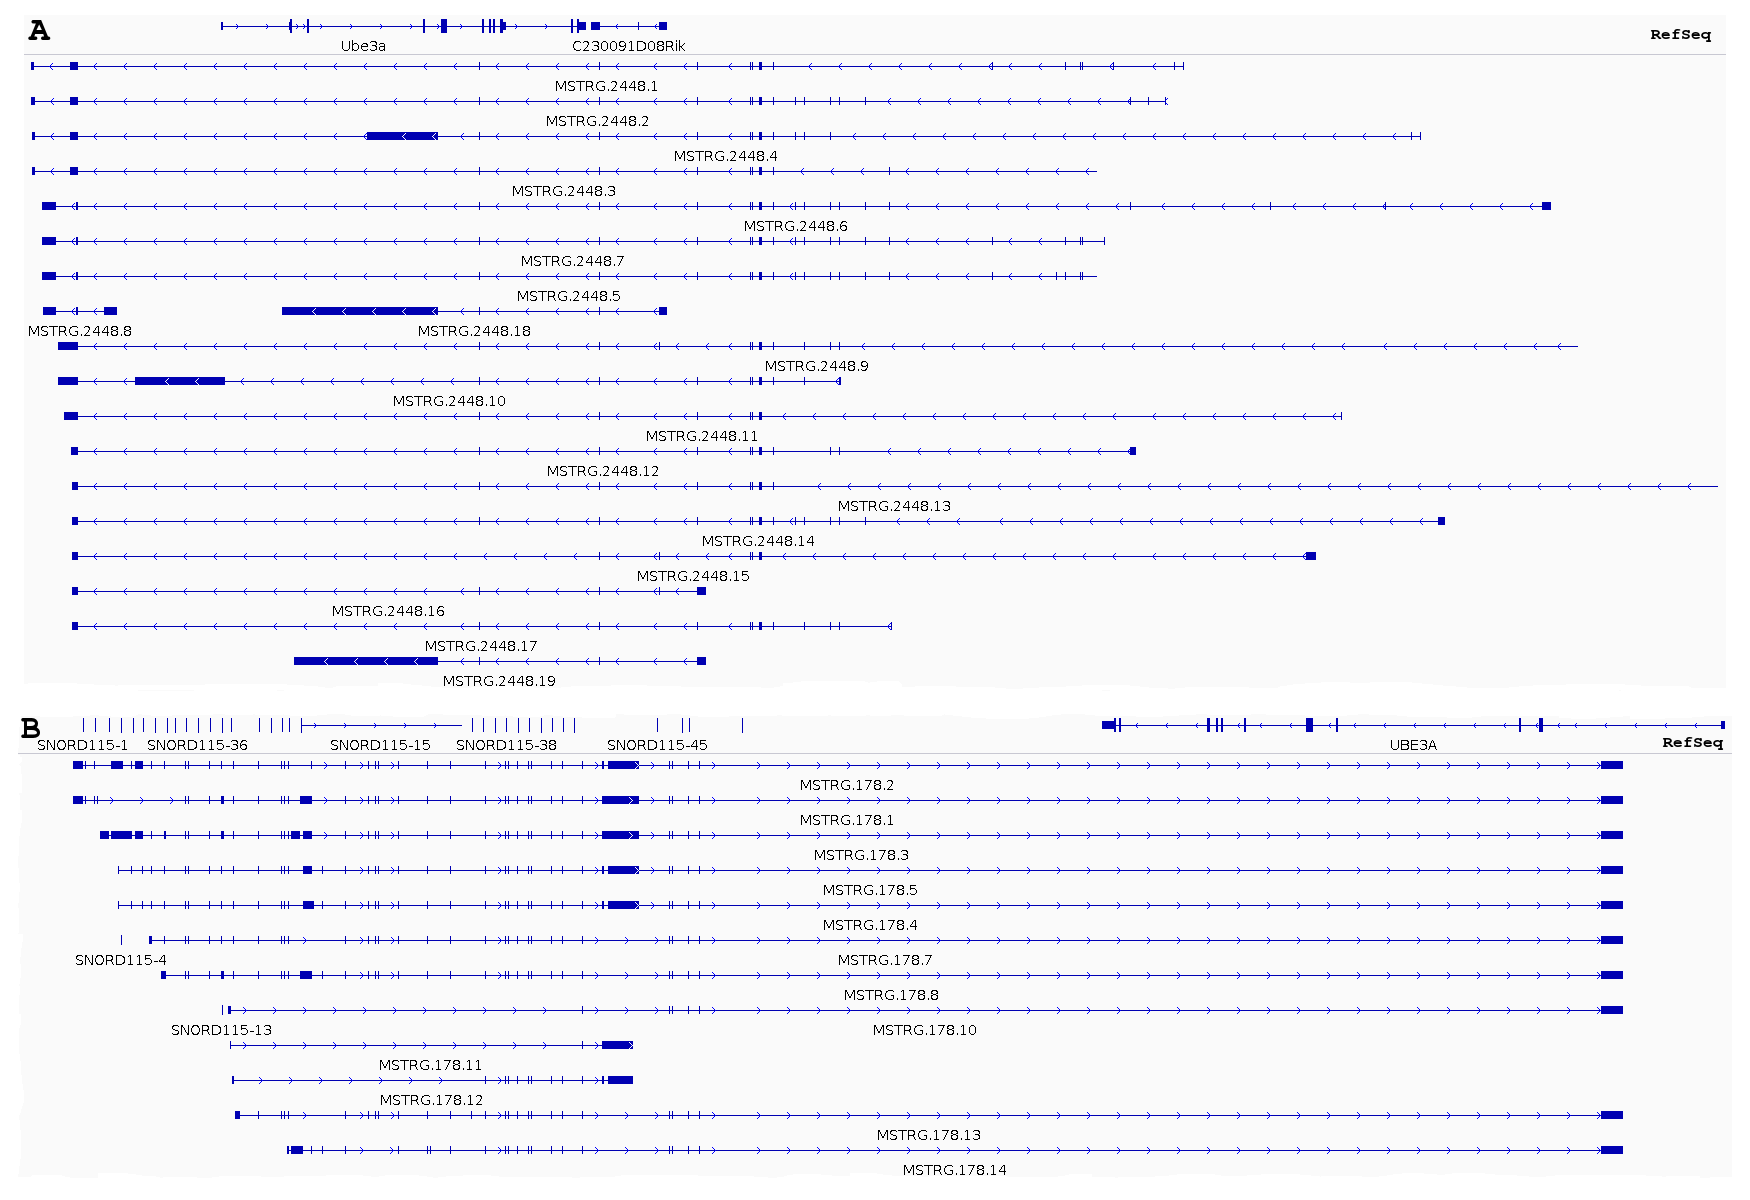
\includegraphics{figures/chapter2.antisense.annotation.png}
  }
  \caption{Antisense transcript of \textit{Ube3a/UBE3A} is alternatively spliced in the brain. \textbf{A.} Schematic of mouse \textit{Ube3a-AS}. Data generated from Pervouchine \textit{et al.} (2015). \textbf{B.} Schematic of human \textit{UBE3A-AS}. Data generated from Lin \textit{et al.} (2016).}
  \label{genome annotation}
\end{sidewaysfigure}
%%%%%%%%%%%%%%%%%%%%%%%%%%%%%%%%%%%%%%%%%%%%%%%%%%%%%%

To investigate processing of the antisense transcripts, we applied publicly available polyA-seq and CAGE-seq in conjunction with 3' RACE (\textbf{Figure \ref{antisense processing}}). In the antisense direction of \textit{UBE3A/Ube3a}, polyadenylation sites were identified with several verified by 3' RACE sequence data (\textbf{APPENDIX B}). Analysis of antisense direction CAGE data revealed 5' capped sites within the antisense region. Combined with the polyadenylation data, this suggested that the antisense transcripts are being processed into smaller RNAs.

As the \textit{UBE3A/Ube3a} region is imprinted, it was important that we identify allelic origin of expression. To this end, the hybrid mice - sequenced by Sanger Institute Collaboration - were used to identify informative SNPs in the region. Of the six SNPs in the region, five of them had approximately 97.8\% expression from the paternal (DBA) allele at $\sim$52.1\% coming from the reverse strand (\textbf{APPENDIX B, Table \ref{snp table1}}. Suggesting that these antisense transcript are being expressed from the paternal allele.

%%%%%%%%%%%%%%%%%%%%%%%%%%%%%%%%%%%%%%%%%%%%%%%%%%%%%%
\begin{sidewaysfigure}
  \centering
  \resizebox{\linewidth}{!}{
    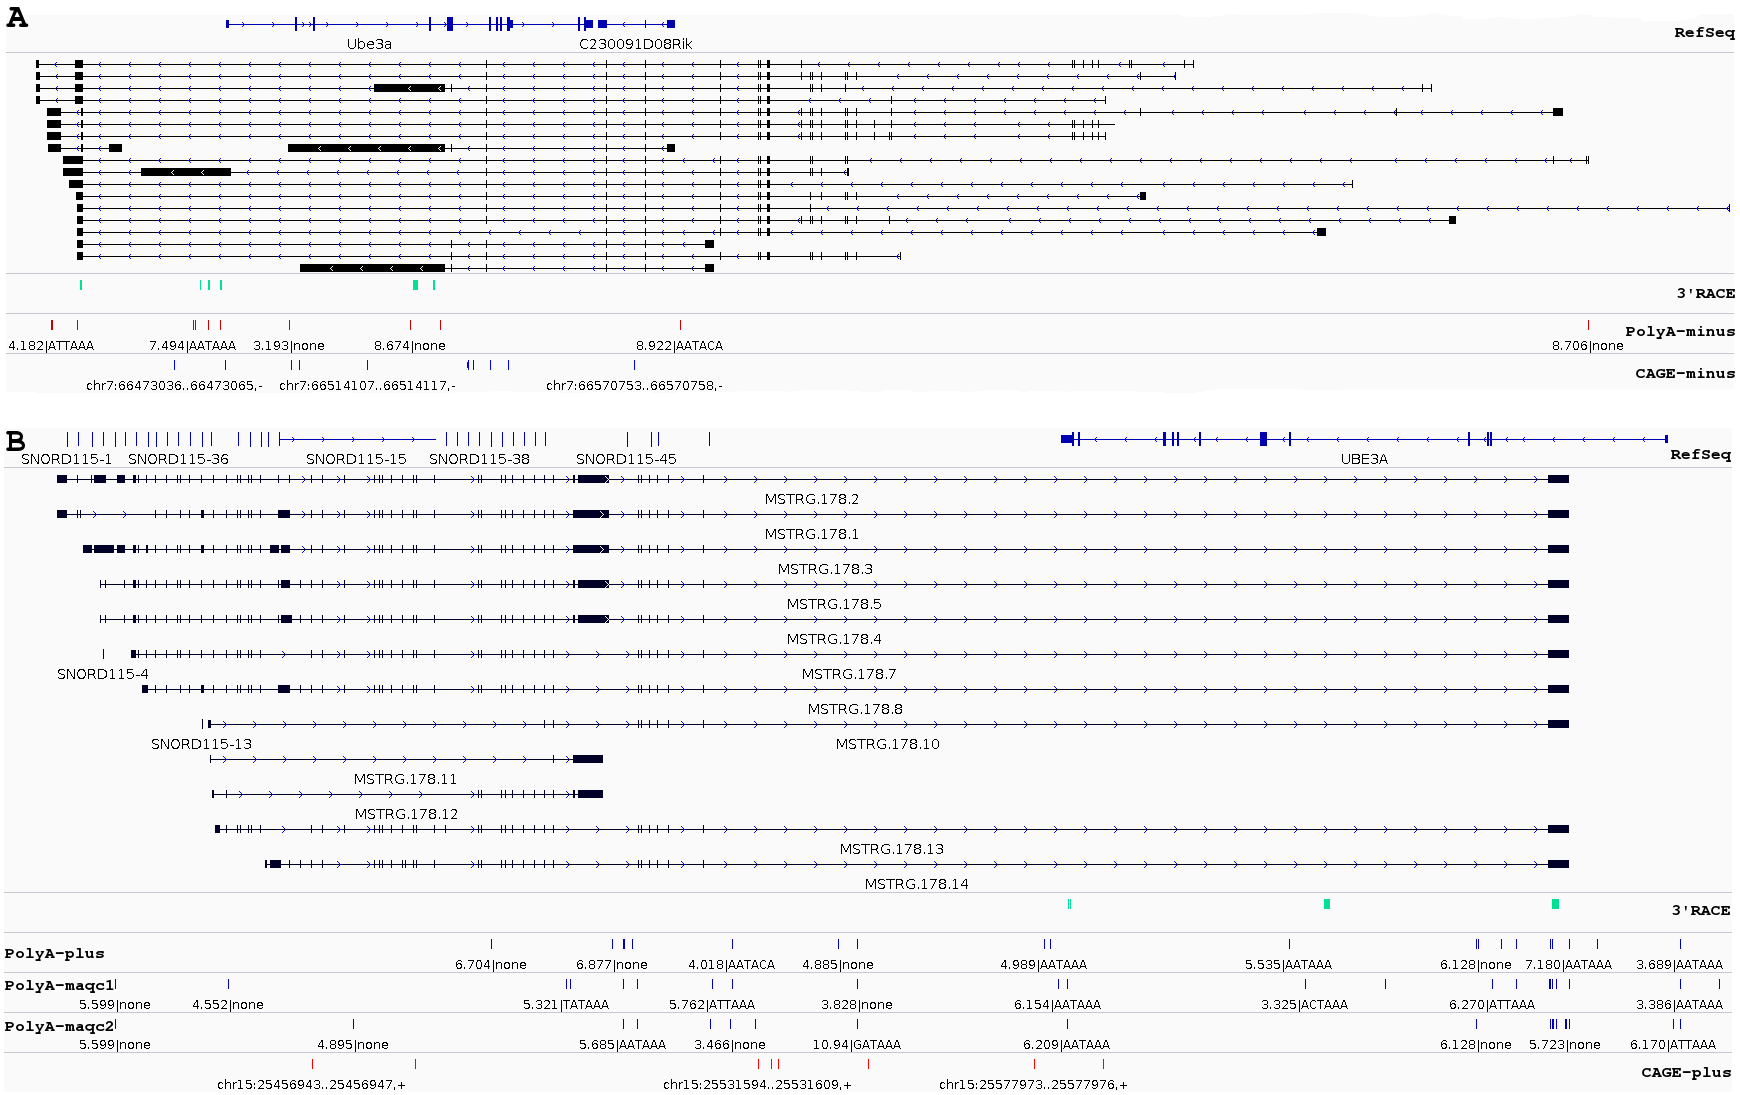
\includegraphics{figures/chapter2.antisense.processing.png}
  }
  \caption{\textit{Ube3a-AS/UBE3A-AS} is extensively processed in the brain. \textbf{A.} Schematic of mouse antisense transcript polyadenylation sites, 5' capping, and 3'RACE confirming several polyA sites. \textbf{B.} Schematic of human antisense transcript polyadenylation, 5' cappin, and 3'RACE. Polyadenylation data generated by Derti \textit{et al.} (2012). 5' capping data generated by Lizio \textit{et al.} (2015).}
  \label{antisense processing}
\end{sidewaysfigure}
%%%%%%%%%%%%%%%%%%%%%%%%%%%%%%%%%%%%%%%%%%%%%%%%%%%%%%

In addition to the 3' and 5' processing of these antisense transcripts, we observed numerous splicing and alternative splicing in the antisense direction with Sashimi plots within the mouse cortex (\textbf{Figure \ref{sashimi brain}A}), and within the human Brodmann area 4 (\textbf{Figure \ref{sashimi brain}B}). 

%%%%%%%%%%%%%%%%%%%%%%%%%%%%%%%%%%%%%%%%%%%%%%%%%%%%%%
\begin{sidewaysfigure}
  \centering
  \resizebox{\linewidth}{4in}{
    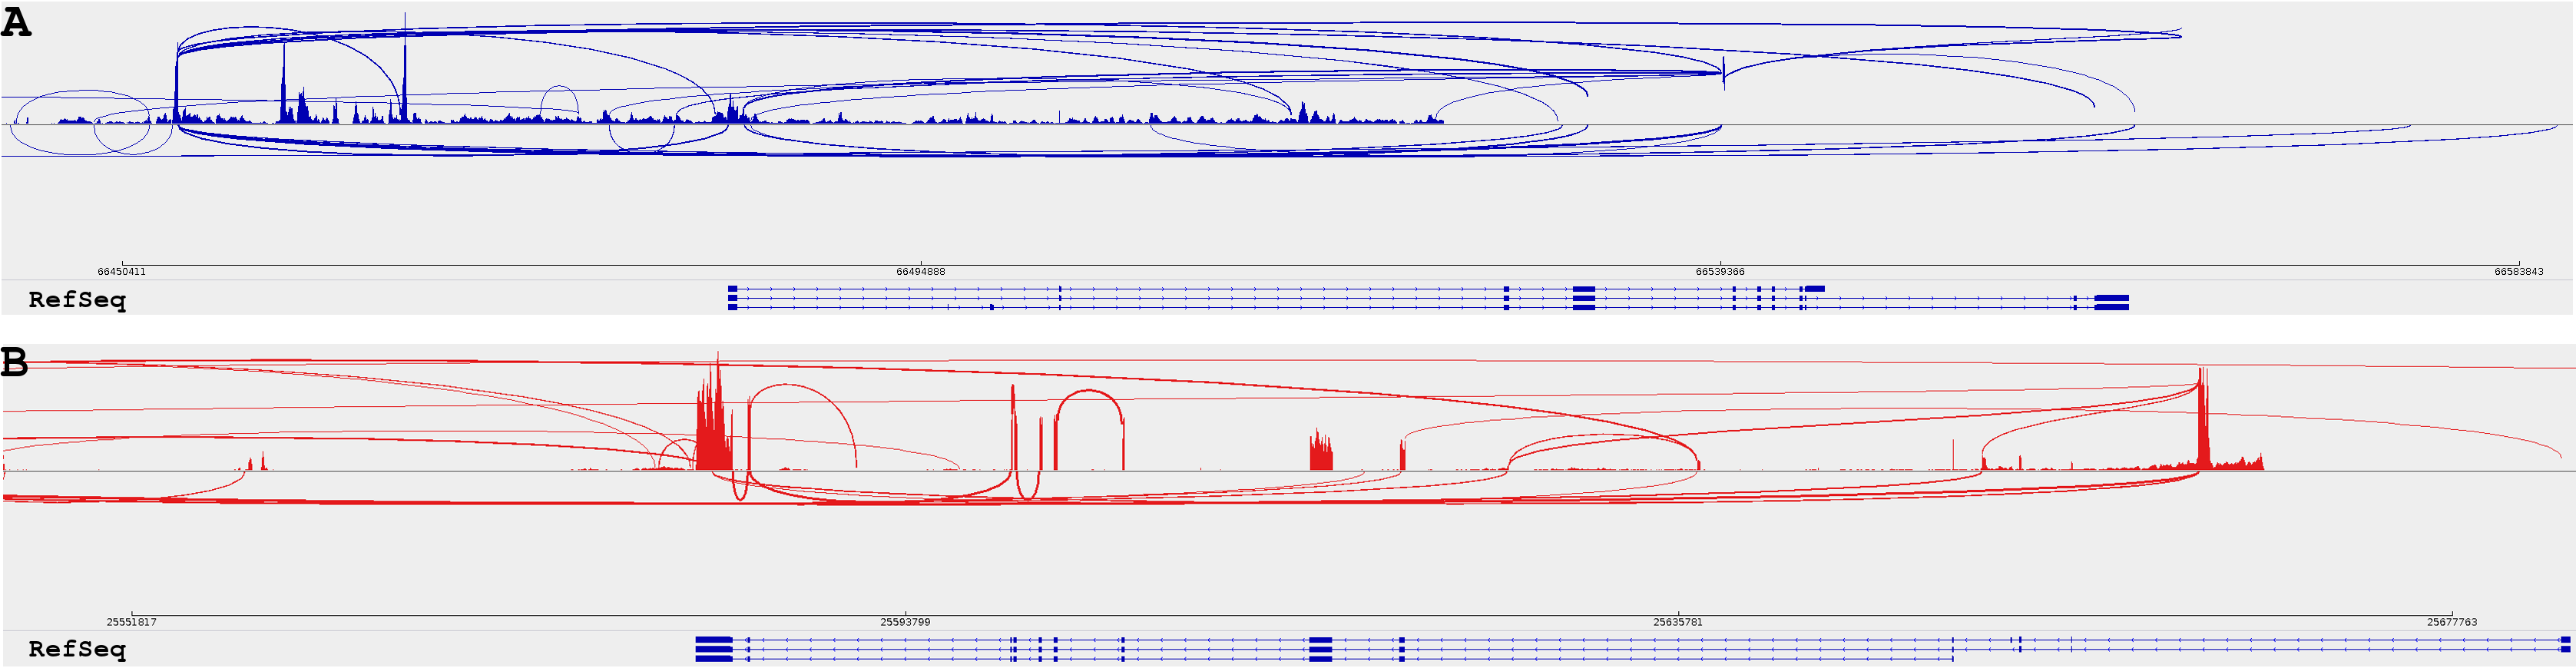
\includegraphics{figures/chapter2.antisense.sashimi.png}
  }
  \caption{Sashimi plots demonstrating numerous splicing and alternative splicing events in the brain of \textbf{A.} mouse (cortex, n = 2) and \textbf{B.} human (BA4, n = 4). Minimum junction coverage = 5. Data generated from Pervouchine \textit{et al.} (2015) and Lin \textit{et al.} (2016).}
  \label{sashimi brain}
\end{sidewaysfigure}
%%%%%%%%%%%%%%%%%%%%%%%%%%%%%%%%%%%%%%%%%%%%%%%%%%%%%%

We used publicly available RNA-seq \cite{Lin2016,Pervouchine2015}, polyA-seq \cite{Derti2012}, CAGE-seq \cite{Lizio2015} data to characterize the expression patterns, splicing, 3' polyadenylation, and 5' capping of the antisense transcript of \textit{UBE3A/Ube3a} in mouse and human. Altogether, these data indicate that the antisense transcripts for mouse and human are processed into multiple transcriptional units through alternative splicing, 5' capping, and 3' polyadenylation. The presence of 5' capped transcripts at exonic and intronic regions also suggests post-transcriptional processing.

\subsection{The \emph{UBE3A-AS/Ube3a-AS} is brain-specific and highly expressed in neurons}

We next examined the expression profile and patterns of the antisense transcript among mouse and human tissues and among individual populations of mouse cerebral cortex cell-types using RNA-seq data \cite{Uhlen2015,Zhang2014}. Alternative splicing in the antisense direction nearly disappeared completely in non-brain tissues in both mouse (\textbf{APPENDIX B, Figure \ref{sashimi tissue specific1}}) and human (\textbf{APPENDIX B, Figure \ref{sashimi tissue specific2}}). Analysis of isoform expression revealed that all of the antisense transcripts were downregulated in heart, liver and lung compared to hippocampus (mouse, \textbf{APPENDIX B, Figure \ref{tissue logFC}A-C}) or cortex (human, \textbf{APPENDIX B, Figure \ref{tissue logFC}D-F}). Similar, \textit{Ube3a-AS} transcripts were all downregulated in astrocytes, OPC (oligodendrocytes precursor cells), NFO (newly formed oligodendrocytes), MO (myelinating oligodendrocytes), microglia, and endothelial cells compared to neurons (\textbf{APPENDIX B, Figure \ref{sashimi celltype anti}}, and \textbf{\ref{logFC celltype anti}}).

As coverage was low for the tissue RNA-seq data, we looked at exon usage between tissues and cell-types of the cerebral cortex to determine significant changes in expression. Three general isoform categories were determined for mouse \textit{Ube3a-AS} based on 3'RACE polyadenylation sites, and one for human \textit{UBE3A-AS} based on 3'RACE polyadenylation (\textbf{Figure \ref{brain specific}A}). Using this method, expression were significantly downregulated compared to the hippocampus in mouse (p-value $<$ 0.001, FDR $<$ 0.001; \textbf{Figure \ref{brain specific}B}), and cortex in human (p-value $<$ 0.001, FDR $<$ 0.001; \textbf{Figure \ref{brain specific}C}) with log2 fold-changes all below -2. Similarly, cell-type expression was also significantly downregulated compared to neurons in mouse (p-value $<$ 0.001, FDR $<$ 0.001; \textbf{Figure \ref{brain specific}D}). Exon genomic position are listed in \textbf{APPENDIX B, Table \ref{exon location table}}.

Altogether, these data demonstrates that the antisense transcript of \textit{Ube3a/UBE3A} is brain-specific, and that \textit{Ube3a-AS} is also highly expressed in neurons compared to other cell-types in the cerebral cortex.

%%%%%%%%%%%%%%%%%%%%%%%%%%%%%%%%%%%%%%%%%%%%%%%%%%%%%%
\begin{figure}
  \centering
  \resizebox{\linewidth}{!}{
    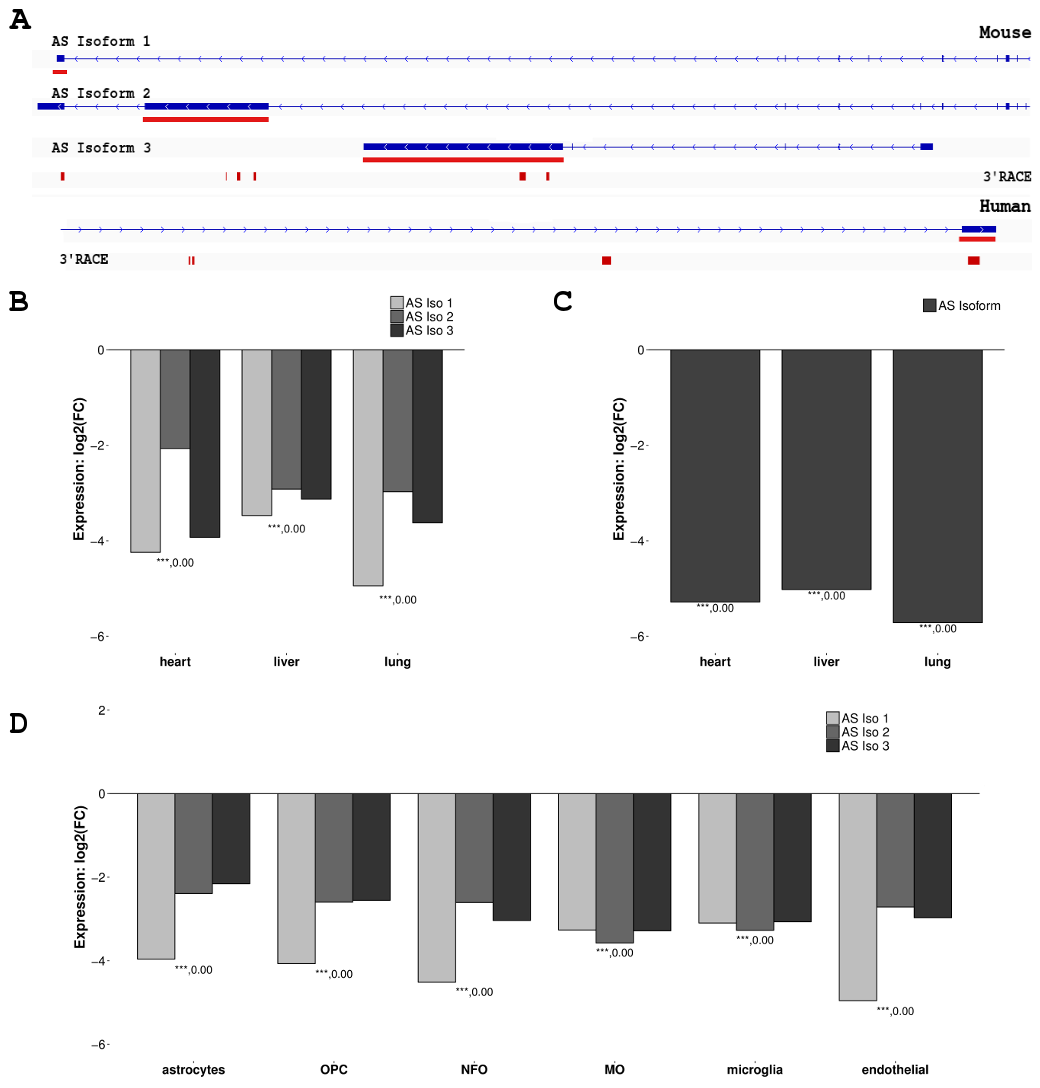
\includegraphics{figures/chapter2.brain-specific2.png}
  }
  \caption{\textit{Ube3a-AS/UBE3A-AS} demonstrates brain-specific differential expression and is upregulated in neurons. \textbf{A.} Schematic of the exons used for differential exon usage comparison. 3'RACE locations marked below annotations. \textbf{B.} Differential expression of \textit{Ube3a-AS} isoforms comparing hippocampus to heart, liver, and lung. Data generated from Sanger Institute hydrid mice data. \textbf{C.} Differential expression of \textit{UBE3A-AS} isoform comparing cortex to heart, liver, and lung. Data generated from Uhlen \textit{et al.} (2015). \textbf{D.} The three mouse isoforms are downregulated in non-neuronal cell-types compared to neurons. Data generated from Zhang \textit{et al.} (2014). P-value and FDR plotted in \textbf{B-C.} *** denotes p-value $<$ 0.001. Abbreviations: OPC - oligodendrocytes precursor cells, NFO - newly formed oligodendrocytes, and MO - myelinating oligodendrocytes.}
  \label{brain specific}
\end{figure}
%%%%%%%%%%%%%%%%%%%%%%%%%%%%%%%%%%%%%%%%%%%%%%%%%%%%%%

\subsection{The \emph{Ube3a-AS} is spatiotemporally regulated}

We next asked whether the antisense transcripts are differentially regulated among brain regions. Using the same general isoforms categories above (\textbf{Figure \ref{brain specific}A}), we looked at the fold-change comparing cortex to cerebellum and frontal lobe, and frontal lobe compared to cerebellum (\textbf{Figure \ref{spatiotemporal regulated}A}). \textit{Ube3a-AS} isoform 1 (AS Iso1) and \textit{Ube3a-AS} isoform 2 (AS Iso2) were significantly downregulated in cerebellum compared to cortex and frontal lobe (p-value $<$ 0.001, FDR $<$ 0.001), while \textit{Ube3a-AS} isoform 3 (AS Iso3) was significantly upregulated in cerebellum compared to cortex and frontal lobe (p-value $<$ 0.001, FDR $<$ 0.001). There appeared to be no difference between cortex and frontal lobe expression, which is unsurprising given their locations in the brain.

To expand upon our findings that \textit{Ube3a-AS} is differentially expressed among mouse brain regions, we used quantitative RT-PCR to examine the levels of the three general isoforms among adult mouse cerebellum, cortex, and hippocampus (C57BL/6, n=3; \textbf{Figure \ref{spatiotemporal regulated}B}). The levels of each transcript were significantly different among the brain regions (ANOVA, F $<$ 0.001), with significantly higher levels of relative expression for AS Iso1 in cortex and hippocampus compared to cerebellum (Tukey's HSD, p.adj $<$ 0.01; p.adj $<$ 0.01). AS Iso3 had significantly higher levels of relative expression in cerebellum compared to cortex or hippocampus (Tukey's HSD, p.adj $<$ 0.001), which supported the RNA-seq analysis. AS Iso2 was virtually undetectable in all brain regions.

In addition to spatial analysis, we also wanted to see if \textit{Ube3a-AS} was regulated during brain development in the hippocampus (\textbf{Figure \ref{spatiotemporal regulated}C}). Using the general isoforms, we examined the fold-change comparing E18 to P1, P10, and P30 finding that AS Iso2 was significantly upregulated in P30 compared to E18 (p-value $<$ 0.01, FDR $<$ 0.05). When comparing P1 to P10 and P30, we found that expression of AS Iso1 was significantly upregulated compared to P10 and P30 (p-value $<$ 0.01, FDR $<$ 0.05), and AS Iso2 was significantly upregulated compared to P30 (p-value $<$ 0.001, FDR $<$ 0.001). AS Iso3 did not appear to be significantly upregulated. 

Altogether, these findings indicate that \textit{Ube3a-AS} is differentially regulated among brain regions and during brain development. 

%%%%%%%%%%%%%%%%%%%%%%%%%%%%%%%%%%%%%%%%%%%%%%%%%%%%%%
\begin{figure}
  \centering
  \resizebox{\linewidth}{!}{
    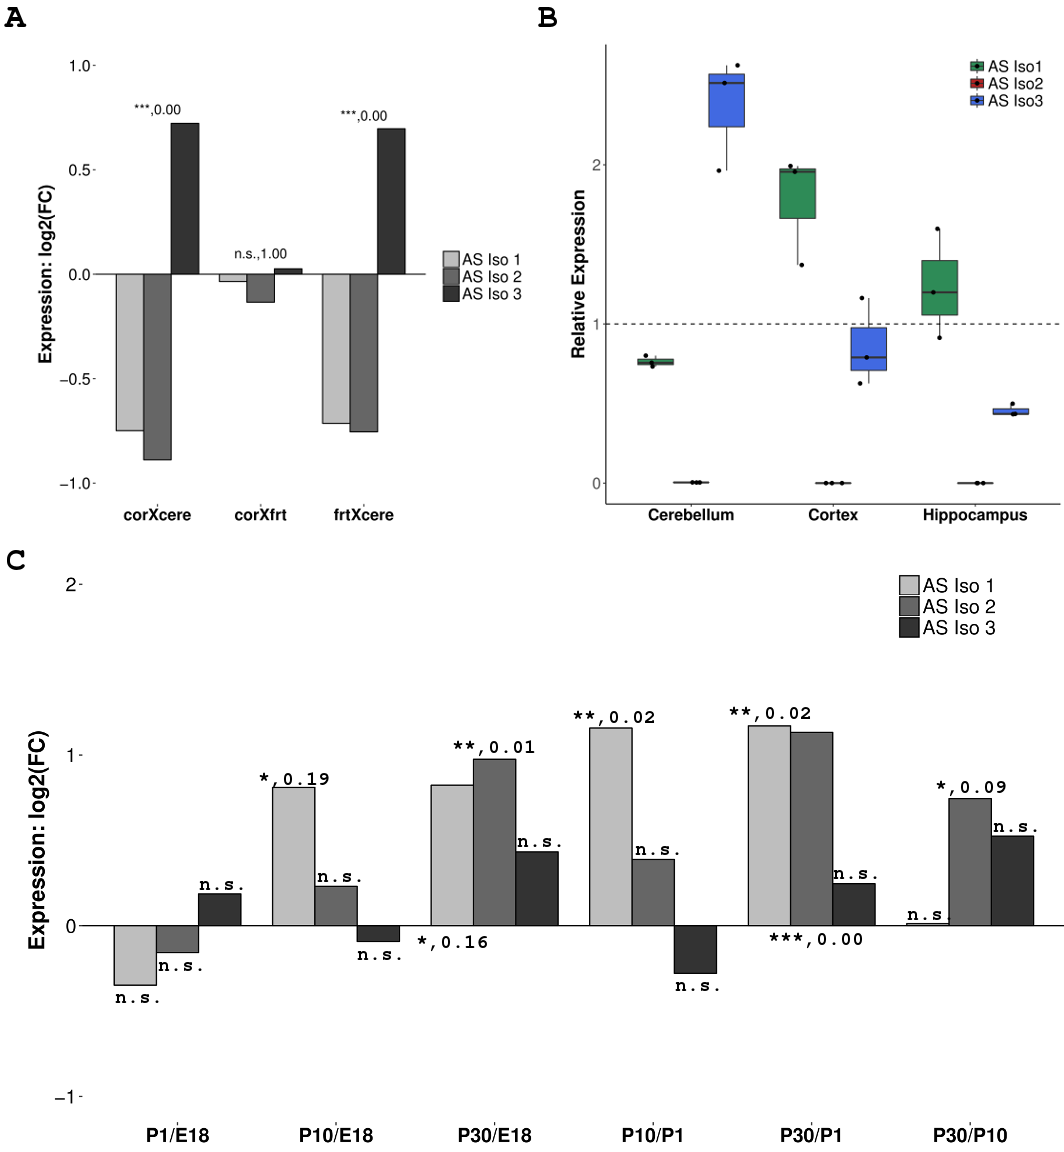
\includegraphics{figures/chapter2.spatiotemporal.png}
  }
  \caption{\textit{Ube3a-AS} is spatiotemporally regulated in the brain. \textbf{A.} Log2 fold-change comparing cortex, cerebellum and frontal lobe (n = 2). Data generated from Pervouchine \textit{et al.} (2015). \textbf{B.} qPCR relative expression comparing isoform expression between cortex, cerebellum and hippocampus (n = 3). \textbf{C.} Log2 fold-change comparing developmental timepoints (E18, P1, P10, and P30) within the hippocampus (n = 2). Data generated from You \textit{et al.} (2015). P-value and FDR ploted in \textbf{A.} and \textbf{C.} *** denotes p-value $<$ 0.001, ** denotes p-value $<$ 0.01, and * denotes p-value $<$ 0.05.}
  \label{spatiotemporal regulated}
\end{figure}
%%%%%%%%%%%%%%%%%%%%%%%%%%%%%%%%%%%%%%%%%%%%%%%%%%%%%%


\section{Discussion}

In this study, we investigated expression profiles of the antisense transcript to \textit{Ube3a/UBE3A}, and determined that the \textit{Ube3a/UBE3A} antisense transcript is extensively processed in the brain with 5' capping, 3' polyadenylation, and alternative splicing. In addition to this, we demonstrated that \textit{Ube3a-AS/UBE3A-AS} is brain-specific, and in mice, upregulated in neurons with paternal exclusive expression. Lastly, we found that \textit{Ube3a-AS} is spatiotemporally expressed. Based on these findings, we propose that \textit{Ube3a-AS/UBE3A-AS} is a highly processed transcript with potential functionality.

Studies to date indicate that the \textit{UBE3A-AS} is transcribed as part of a long polycistronic transcriptional unit on the paternal chromosome \cite{Chamberlain2001,Landers2004,Runte2001}. Our results are consistent with this theory (\textbf{APPENDIX B, Figure \ref{mean expression-ballgown}}); furthermore, we found that several of transcripts assembled were highly interconnected with the upstream \textit{Snord115/SNORD115} gene. Additionally, we did not observe any 5' capping near the predicted 5' ends of the mouse antisense transcripts. The presence of 5' capped transcripts in \textit{Ube3a-AS/UBE3A-AS} region lacked an active transcriptional start site and aligned either to exonic or intronic regions suggesting post-transcriptional modifications \cite{Affymetrix2009,Kiss2015,Mercer2010}. Furthermore, we identified and verified polyadenylation sites throughout both intronic and exonic regions of \textit{Ube3a-AS/UBE3A-AS}. Altogether suggesting that the region is transcribed as 5' capping and 3' polyadenylation are often coupled with transcription to prevent degradation of the RNA transcript, facilitate nuclear export, and/or promote translation \cite{Hocine2010}.

We also confirm that the \textit{Ube3a-AS/UBE3A-AS} is primarily, if not exclusively, expressed in the brain. Splicing in the antisense direction was almost completely eliminated in non-brain tissues. Furthermore, upon examination of differential expression in cerebral cortex cell populations, we observed a drastic decrease in splicing in non-neuronal cell-types that are consistent with previous studies that imprinting of \textit{Ube3a} is neuron-specific \cite{Dindot2008,Yamasaki2003}.
By using exon level differential expression, we were able to see log2 fold-changes greater than 2, which was not apparent with transcript level differential expression. This could be due to the overlapping regions of \textit{Ube3a/UBE3A} and the antisense transcripts. As such, general antisense isoforms were chosen near the 3' ends of the antisense transcript where 3'RACE had confirmed the polyadenylation site. Interestingly, these isoforms appeared to also be differentially expressed within tissue and cell-type comparisons with isoform 1 having the, overall, highest differential expression.

In addition to being differentially expressed, we determined that the \textit{Ube3a-AS} isoforms were also spatially regulated within the brain with isoform 3 begin upregulated in cerebellum, and isoform 1 and 2 upregulated in cortex, frontal lobe, and hippocampus. Furthermore, we determined that \textit{Ube3a-AS} was also temporally regulated in the hippocampus with expression of isoform 1 during the P1 developmental time period. This was of interest as \textit{Creb3l1} - a cAMP protein, \textit{Kcnd2} - a potessium voltage-gated channel protein, \textit{Stx3} - a syntaxin protein, and \textit{Slc6a4} - a neurotransmitter protein are also temporally regulated in the brain at the P1 stage \cite{BrainScience2008,Sunkin2012}. Isoform 2 expressing during the P10 time period, where several enhancers and transcription factors like \textit{Hes3} and \textit{Atf6} are also temporally regulated in the brain \cite{BrainScience2008,Sunkin2012}. We did not observe temporal regulation with isoform 3; however, as the tissue examined was hippocampal and isoform 3 showed significant upregulation in the cerebellum tissue. As such, it is possible that isoform 3 could be temporally regulated in the cerebellum. 

Altogether, these findings provide insight into the function of the \textit{UBE3A-AS} and the function of neuron-specific imprinting of \textit{UBE3A}. Processing of mRNA and ncRNA to generate shorter RNA transcripts often expand the functional capacity of the transcriptome, generating shorter RNAs and in some instances isoforms with coding potential. Here, we propose that \textit{UBE3A-AS} is expressed in neurons for a regulatory function outside of the imprinting of \textit{UBE3A}. Furthermore, these new insights offer clues as to how the antisense can be targeted for therapeutic intervention and raises potential ramifications of doing so.
